%
% mismatch.tex -- mismatch of boundary conditions for y''=0
%
% (c) 2019 Prof Dr Andreas Müller, Hochschule Rapperswil
%
\documentclass[tikz,12pt]{standalone}
\usepackage{amsmath}
\usepackage{times}
\usepackage{txfonts}
\usepackage{pgfplots}
\usepackage{csvsimple}
\usetikzlibrary{arrows,intersections,math}
\begin{document}
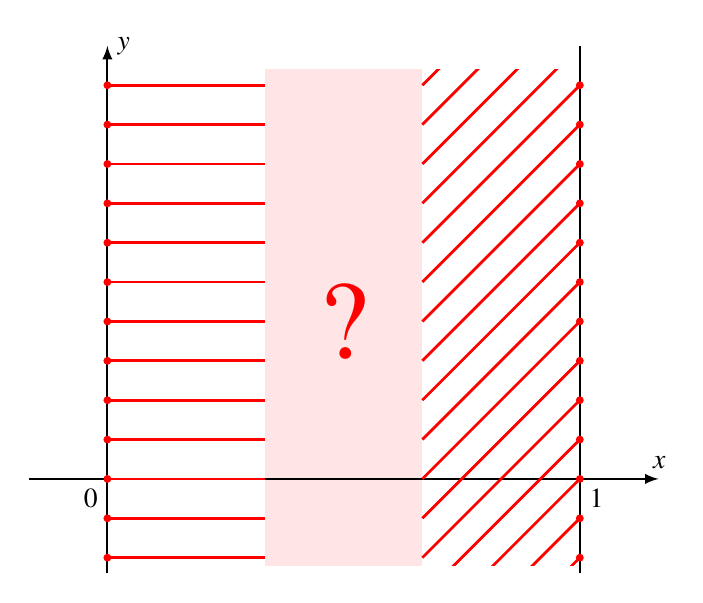
\begin{tikzpicture}[>=latex]

\fill[color=red!10] (2,-1.1) rectangle (4,5.2);

\draw[->,line width=0.7pt] (-1,0)--(7,0) coordinate[label={$x$}];
\draw[->,line width=0.7pt] (0,-1.2)--(0,5.5) coordinate[label={right:$y$}];
\draw[line width=0.7pt] (6,-1.2)--(6,5.5);

\begin{scope}
\clip (-0.2,-1.1) rectangle (6.1,5.2);
\foreach \y in {-2,-1.5,...,7}{
	\fill[color=red] (0,{\y}) circle[radius=0.05];
	\fill[color=red] (6,{\y}) circle[radius=0.05];
	\draw[color=red,line width=1pt] (0,{\y})--(2,{\y});
	\draw[color=red,line width=1pt] (6,{\y})--(4,{\y-2});
}
\end{scope}

\node[scale=4,color=red] at (3,2) {?};

\node at (0,0) [below left] {$0$};
\node at (6,0) [below right] {$1$};

\end{tikzpicture}
\end{document}

